% HW Template for CS 6150, taken from https://www.cs.cmu.edu/~ckingsf/class/02-714/hw-template.tex
%
% You don't need to use LaTeX or this template, but you must turn your homework in as
% a typeset PDF somehow.
%
% How to use:
%    1. Update your information in section "A" below
%    2. Write your answers in section "B" below. Precede answers for all 
%       parts of a question with the command "\question{n}{desc}" where n is
%       the question number and "desc" is a short, one-line description of 
%       the problem. There is no need to restate the problem.
%    3. If a question has multiple parts, precede the answer to part x with the
%       command "\part{x}".
%    4. If a problem asks you to design an algorithm, use the commands
%       \algorithm, \correctness, \runtime to precede your discussion of the 
%       description of the algorithm, its correctness, and its running time, respectively.
%    5. You can include graphics by using the command \includegraphics{FILENAME}
%
\documentclass[11pt]{article}
\usepackage{amsmath,amssymb,amsthm}
\usepackage{graphicx}
\usepackage[margin=1in]{geometry}
\usepackage{fancyhdr}
\usepackage{framed}
\usepackage{algorithm}
\usepackage{algpseudocode}
\usepackage{pifont}
\setlength{\parindent}{0pt}
\setlength{\parskip}{5pt plus 1pt}
\setlength{\headheight}{13.6pt}
\newcommand\question[2]{\vspace{.25in}\hrule\textbf{#1}\vspace{.5em}\hrule\vspace{.10in}}
\renewcommand\part[1]{\vspace{.10in}\textbf{(#1)}}
\newcommand\algorith{\vspace{.10in}\textbf{Algorithm: }}
\newcommand\correctness{\vspace{.10in}\textbf{Correctness: }}
\newcommand\runtime{\vspace{.10in}\textbf{Running time: }}
\pagestyle{fancyplain}
\lhead{\textbf{\NAME\ (\UID)}}
\chead{\textbf{HW\HWNUM}}
\rhead{CS 6490, \today}
\begin{document}\raggedright
%Section A==============Change the values below to match your information==================
\newcommand\NAME{Jake Pitkin}  % your name
\newcommand\UID{u0891770}     % your utah UID
\newcommand\HWNUM{4}              % the homework number
%Section B==============Put your answers to the questions below here=======================

\question{Question 1}

\textbf{Suppose a computer is authenticated based on its IP address (no passwords are used). Identify one strength and one weakness of such an authentication mechanism.}

\textit{Strength:} With an address-based authentication, passwords don't need to be created, remembered, or passed around the network. This makes addressed-based authentication much more convenient than password-based systems. Additionally, passwords can't be intercepted by eavesdroppers, brute force guessed using rainbow tables, or leaked as the result of a compromised database.

\textit{Weakness:} Trudy can impersonate Alice's network address and pose as her on the network. She can perform source routing and inject IP packets to route traffic in such a way that she can transmit from and receive packets for Alice's network address. This comes with it's share of complications (additional cryptographic authentication on the router), as most security threats do.

\question{Question 2}

\part{a} \textbf{Problem 2, Chapter 9, page 236.}

The described scheme guards against eavesdropping but is \textbf{vulnerable to server database disclosure}.

It's secure against eavesdropping as the information Trudy can intercept is: who is trying to authenticate (Alice), a random number R, and the hash of Alice's password and R. Assuming R is sufficiently random and not repeated, $hash(Y,R)$ will not be repeated so this is of no use to Trudy.

However it vulnerable against server database disclosure. Assume Trudy gains access to the database and it contains a table of usernames to hashed passwords for that user. Now Trudy can say to Bob "I'm Alice" and Bob will send Trudy R. Trudy now knows Z (hash of Alice's password) and can compute $hash(Z,R)$ and respond to Bob. Bob will check if this matches $hash(Z,R)$ (which it will) and authenticate Trudy as Alice. 

\part{b} \textbf{Let a dictionary have 4,096 words. Let a user pick 5 words at random for choosing a password (i.e., the password comprises of these 5 words). What is the strength of this password in bits?}

To represent 4,096 words in binary it will require 12-bits. This is because $4,096 = 2^{12}$. As such, each randomly picked word will provide 12-bits of randomness to the password. Since the user chooses 5 words at random, we will concatenate the bit patterns and provide \textbf{60-bit security}.

\question{Question 3}

\part{a} \textbf{Could $\mathbf{f(K_{AB}, R)}$ be a secure hash function of $\mathbf{K_{AB}}$ and R in the protocol below? Explain briefly.}

The protocol is not secure, it is susceptible to an off-line dictionary attack by an eavesdropper. 

Trudy can eavesdrop in on Alice and Bob and obtain a set of $f(K_{AB}, R)$ and $R$. Now Trudy can go off-line and use brute force to obtain $K_{AB}$. She can generate a guess for Alice and Bob's secret key $K_{G}$ and apply the hash function $f$ to it and $R$. She checks if $f(K_{G}, R) = f(K_{AB}, R)$ and when it does she has found their secret key.

\part{b} \textbf{Give two reasons why should we use different keys for different purposes?}

\textit{Reason 1:} If Alice and Bob use a shared secret key to authenticate each other in a naive way, they are susceptible to a \textbf{reflection attack}. 

Say Alice sends a nonce $R1$ to Bob and Bob responds with $f(K_{AB}, R1)$ and $R2$ (his own nonce). Bob is expecting $f(K_{AB}, R2)$ back from Alice which she can produce since she has $K_{AB}$.

But consider how Trudy can take advantage of this. Trudy can open a first connection with Bob, saying she is Alice, and send a nonce $R1$. Bob responds with $f(K_{AB}, R1)$ and $R2$; he is waiting for $f(K_{AB}, R2)$. 

Trudy opens a second connection with Bob and sends $R2$ (the same nonce Bob sent her in connection 1) and Bob responds with $f(K_{AB}, R2)$ and $R3$. Finally Trudy goes back to connection 1 and sends Bob $f(K_{AB}, R2)$ and authenticate as Alice with never knowing $K_{AB}$. As such, we shouldn't use the same keys for both directions of authentication.

\textit{Reason 2:} Using separate private keys for signing messages and authentication. As we saw in class, one way Bob can authenticate Alice is to send Alice a nonce $R$. Alice will authenticate herself by signing the nonce with her private key $A^-\{R\}$. The problem here is anyone can now send Alice a message (disguised as a nonce) and have her sign it.

There is a similar problem with encrypting the nonce $R$ with Alice's public key $A^+\{R\}$ and having her decrypt it as authentication. Now anyone can send Alice a ciphertext she previously produced with her public key and get her to decrypt it. 

\part{c} \textbf{What is the problem when session key establishment to protect the rest of the session does not follow an authentication protocol? Explain briefly.}

There are a number of things that can go wrong if session key establishment does not follow a secure authentication protocol. If the session key is not secure, the rest of the session will not be secure.

\textit{Authenticate as Alice:} Trudy can pose as Alice and initiate a conversation with Bob. As seen in question (3b), Trudy can perform a reflection attack and authenticate to Bob as Alice if the protocol isn't secure.

\textit{Session Hijacking:} In the worst case the session key is plainly transmitted over the connection between Alice and Bob. An eavesdropper can obtain this key and hijack the session, posing as either party. In a slightly more secure (but still vulnerable) protocol, enough information is transmitted for Trudy to perform an off-line dictionary attack to obtain the key. An example of this is question (3a).

\part{d} \textbf{What would be a good session key between Alice and Bob following the authentication exchange (shown below) such that (i) even if an adversary obtains the key, it cannot find $\mathbf{K_{AB}}$, and (ii) the session key is unique for every session?}

A good session key for Bob and Alice would be $(K_{AB} + 1)\{R\}$. That is, the challenge $R$ is encrypted with ($K_{AB} + 1$) as the key.

(i) Even if the adversary obtains the session key $K_{AB}+1\{R\}$, they cannot find $K_{AB}$. An offline dictionary attack on the session key and $R$ would not produce $K_{AB}$ even if they were able to brute force it.

(ii) The session key will be unique for every session assuming the nonce $R$ is sufficiently large and the encryption method used to produce the session key is strong.

\part{e} \textbf{Consider the one-way authentication protocol shown in the figure below. Here, Bob is a stateless server, and therefore it is inconvenient to require him to remember the challenge he sent to Alice. Let $\mathbf{K_{AB}}$ be the secret key shared between Alice and Bob. Now, this protocol is vulnerable to a replay attack where an eavesdropper can record R, $\mathbf{K_{AB}\{R\}}$ pair and replay that later. If we enhance the protocol such that R represents the current time, is the protocol secure? Identify one strength, and one weakness of this enhanced protocol.}

\textit{Strength:} I am going to assume Bob is now only accepting timestamps within a certain window of the current time. As such, an adversary would have to be very quick to eavesdrop in on the conversation, obtain $R$ $K_{AB}\{R\}$ and conduct a replay attack.

\textit{Weakness:} This enhanced protocol is still vulnerable to an off-line dictionary attack. The pairs $R$, $K_{AB}\{R\}$ are available to an eavesdropper which they can use to take off-line guesses at $K_{AB}$. Once Trudy has $K_{AB}$ she can authenticate as Alice.

\part{f} \textbf{In the discussion of Protocol 11-3 on page 261, Bob remembers all the timestamps he's seen within the last 10 minutes. Why is this sufficient for him to remember only 10 minutes worth of timestamps?}

In Protocol 11-3, Alice uses the shared key between her and Bob $K_{AB}$ and encrypts the current timestamp $K_{AB}(timestamp)$. She sends this value to Bob, Bob decrypts the result and checks if the $timestamp$ is within a reasonable clock skew window (let's say 10 minutes).

Bob remembers all of the $timestamps$ he has encountered in the last 10 minutes. This is to prevent an eavesdropper from sniffing $K_{AB}(timestamp)$ and attempting to reuse the value and authenticate as Alice.

Bob only has to remember $timestamps$ he has seen in the last 10 minutes because any $timestamp$ outside of the clock skew window is invalid and rejected, even if it is genuinely from Alice.

\part{g} \textbf{Design a two-message authentication protocol, assuming that Alice and Bob know each other's public keys, which accomplishes both mutual authentication and establishment of a session key.}

Consider the following two-message authentication protocol:

\begin{figure}[H]
  \centerline{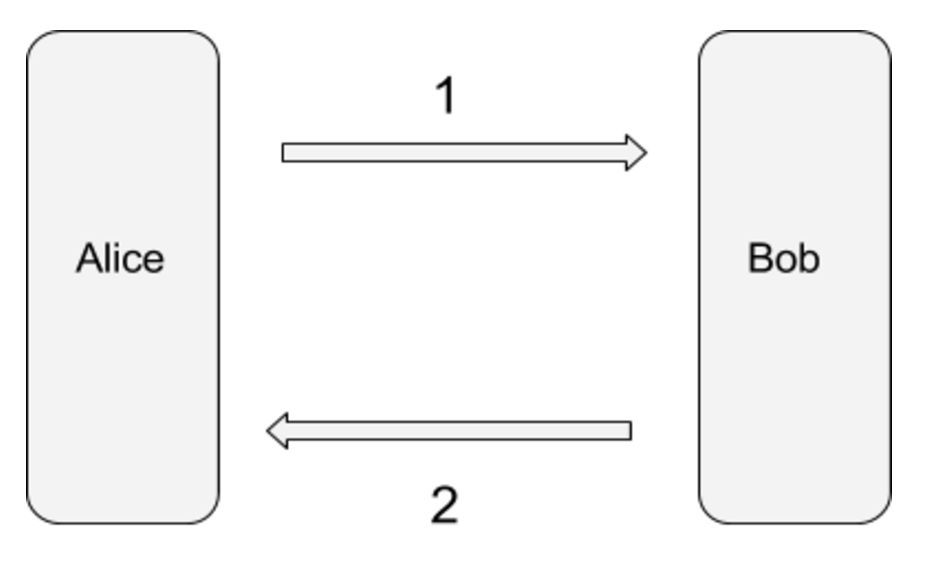
\includegraphics[width=0.5\linewidth]{protocol.png}}
\end{figure}

\textbf{1:} Alice generates a random session key $K_{AB}$ and a nonce $R1$. Alice uses her private key $A^-$ to sign a message consisting of $K_{AB}$ and $R1$ encrypted with Bob's public key $B^+$. The signature of the message (using the standard RSA signature method of hashing the message) and the message are sent to Bob.
$$m = B^+(K_{AB}, \ R1)$$
$$A^-(m), \ m$$

\textbf{2:} Bob receives Alice's signature and message. Bob uses Alice's public key $A^+$ and an identical hashing function to verify the message is from Alice. Bob uses his private key $B^-$ to decrypt $K_{AB}$ and $R1$ from $B^+(K_{AB}, \ R1)$. Bob uses $K_{AB}$ to encrypt $R1$ and sends $K_{AB}\{R1\}$ to Alice.

Finally Alice uses $K_{AB}$ to decrypt $K_{AB}\{R1\}$ and verifies $R1$ is correct.

\textbf{Security:} Bob knows $m = B^+(K_{AB}, \ R1)$ is genuinely from Alice because Alice has signed $m$. If an adversary attempts to modify $m$ during transmission, the signature will not agree and Bob will know there is an intruder.

Alice knows Bob is authentic as well. Only someone with Bob's private key can decrypt $K_{AB}$ and $R1$ from $B^+(K_{AB}, R1)$. Alice will know there is an intruder if Bob's response message $K_{AB}\{R1\}$ doesn't agree with the $K_{AB}$ and $R1$ she generated.

\part{h} \textbf{With the help of figures and message exchanges, show the reflection attack on the following protocol:}

\begin{figure}[H]
  \centerline{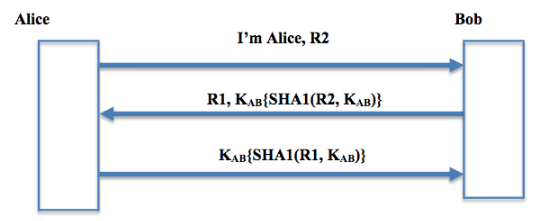
\includegraphics[width=0.5\linewidth]{3h_1.png}}
\end{figure}

For Trudy to perform a reflection attack she will open two connections with Bob, posing as Alice in both. She will open a first connection (Trudy 1) and send a nonce $R2$.

\begin{figure}[H]
  \centerline{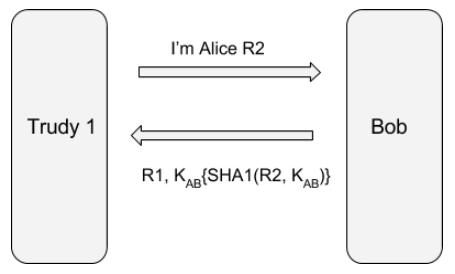
\includegraphics[width=0.5\linewidth]{3h_2.png}}
\end{figure}

Now Bob is expecting $K_{AB}\{SHA1(R1, K_{AB})\}$, so Trudy will open a second connection (Trudy 2) and send the nonce $R1$ she got from Bob.

\begin{figure}[H]
  \centerline{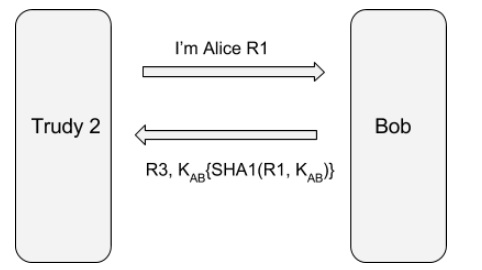
\includegraphics[width=0.5\linewidth]{3h_3.png}}
\end{figure}

Now Trudy has obtained $K_{AB}\{SHA1(R1, K_{AB})\}$, so she will return to connection 1 and reply to Bob.

\begin{figure}[H]
  \centerline{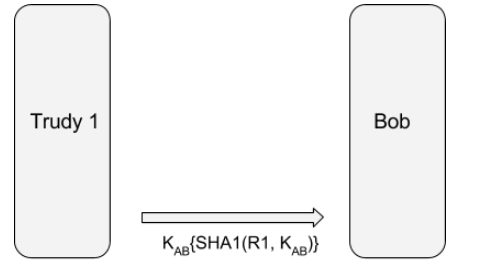
\includegraphics[width=0.5\linewidth]{3h_4.png}}
\end{figure}


\textbf{Here $\mathbf{K_{AB}}$ is the shared secret between Alice and Bob, R1 and R2 are random nonces (random numbers used only once), and the function f is a secret key function or a hash function. The protocol of this question is vulnerable to an off-line dictionary attack by Trudy impersonating as Alice. Modify this protocol appropriately to remove this vulnerability.}

This protocol is vulnerable to a dictionary attack as Trudy can obtain a $R2$, $K_{AB}\{SHA1(R2, K_{AB})\}$ pair by simply posing as Alice and sending a nonce $R2$. Trudy can keep iterating through a dictionary of $K_i$'s, compute $K_{i}\{SHA1(R1, K_{i})\}$ and continue until $K_{x}\{SHA1(R1, K_{x})\}$ is equal to $K_{AB}\{SHA1(R1, K_{AB})\}$ at which point she has found $K_{AB}$.

One solution would be for Alice to use RSA to sign an encrypted version of her original message, sending the message and the signature.

\begin{figure}[H]
  \centerline{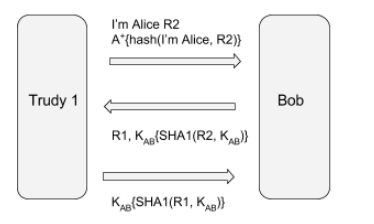
\includegraphics[width=0.5\linewidth]{3h_5.png}}
\end{figure}

Where $A^+$ is Alice's public key. If Alice's signature doesn't prove to be authentic, then Bob will not respond with his second message $R1$, $K_{AB}\{SHA1(R2, K_{AB})\}$. Trudy can't sign a nonce with her own private key, because the response will be encrypted using $K_{TB}$ (Trudy and Bob's shared key assuming they have one).


\question{Question 4}

\part{a} \textbf{Suppose we are using Lamport's hash, and Bob crashes before receiving Alice's reply. Suppose an intruder, Trudy, can eavesdrop and detect that Bob crashed (maybe Trudy can even cause Bob to crash). Then Trudy has a quantity (whatever Alice replied that Bob did not receive) which Trudy can use to impersonate Alice, if Trudy logs in before Alice attempts to log into Bob again. How can we modify Bob's behavior to prevent this threat? (Exactly when do we overwrite Bob's database, and with what)?}

Suppose Alice has initiated wanting to talk to Bob and Bob has responded with $n$. Bob crashes as Alice is responding with $hash^{n-1}(password)$ and Trudy intercepts it. Now, when Bob reboots, Trudy sits between Alice's workstation and Bob posing as Alice. Trudy says she wants to talk, Bob sends $n$, Trudy responds with $hash^{n-1}(password)$, and Trudy is now logged into Bob.

This can be prevented by changing when Bob updates his stored pair for Alice $<n, \ hash^n(password)>$. Normally Bob updates this to $<n-1, \ hash^{n-1}(password)>$ after authenticating Alice. But to make this system less vulnerable to crashes, Bob should update to $<n-1, \ hash^{n-1}(password)>$ \textbf{right before sending n}. And Bob no longer hashes the incoming password before comparing to what he has on record.

Let's say Bob sends $n = 5$ when he crashes so Trudy intercepts Alice's response of $hash^{4}(password)$. Now when Trudy impersonates Alice, Bob will send $n = 4$ and Trudy will have to produce $hash^{3}(password)$. Trudy can't "undo" a hash and produce $hash^{3}(password)$ (as it's a one way function) so she will fail to authenticate.

\part{b} \textbf{Consider Protocol 12-8. How would Alice compute K? How would Bob compute K? Why is it insecure? (Hint: someone impersonating Bob can do a dictionary attack, but show how.)}

\textit{How Alice computes K:} After the initial two exchanges, Alice now has $g^b \ mod \ p$, $a$, and $W$. To compute K Alice will compute the following:

$$K = hash((g^b \ mod \ p)^a \ mod \ p, (g^b \ mod \ p)^W \ mod \ p)$$

We proved in homework 3 that $(x^c \ mod \ n)^d \ mod \ n = x^{cd} \ mod \ n$. We will apply this:

$$K = hash(g^{ab} \ mod \ p, g^{bW} \ mod \ p)$$

And Alice has computed K.

\textit{How Bob computes K:} Bob will compute K in a similar manner. After the initial two exchanges, Bob has $g^W \ mod \ p$, $g^a \ mod \ p$, and $b$. He computes the following:

$$K = hash((g^a \ mod \ p)^b \ mod \ p, (g^b \ mod \ p)^W \ mod \ p)$$

Applying the proven property from homework 3:


$$K = hash(g^{ab} \ mod \ p, g^{bW} \ mod \ p)$$

Now Bob has computed K as well.

\textit{Dictionary attack:} Consider Trudy impersonating as Bob. First, Alice will send Trudy "Alice", $g^a \ mod \ p$. Next Trudy can choose her own $b$ and send Alice $g^b \ mod \ p$ and a challenge $c_1$. Alice will respond with $K\{c_1\}, c_2$.

At this point Trudy knows $g^a \ mod \ p$, $g^b \ mod \ p$, $b$, and $p$ as it's public information. Additionally she has the pair $K\{c_1\}$, $c_1$ will be used to check her offline dictionary attack. Trudy wants to compute K:

$$K = hash(g^{ab} \ mod \ p, g^{bW} \ mod \ p)$$

Notice the only information she doesn't have is $W$. Let $X$ be each of Trudy's offline guesses, the following is an equivalent formula:

$$K = hash((g^a \ mod \ p)^b \ mod \ p, (g^b \ mod \ p)^X \ mod \ p)$$

As such, Trudy will pick an $X$, compute $K$, and use the $K\{c_1\}$, $c_1$ pair to see if she is correct. She will continue until she finds it and finally respond to Alice with $K\{c_2\}$.


\question{Question 5}

\part{a} \textbf{Let us plot the observed clock offset, in microseconds, on the y-axis and the time since the start of the finger printing measurements, in seconds, at the fingerprinter, on the x-axis. Let (6, 60) and (8, 85) be two points at times 6s and 8s, where the clock offset is observed by the fingerprinter to be 60 and 85, respectively. Estimate the clock skew of the fingerprintee from these two points. You can assume that the network delays are negligible.} 

From the paper, the clock skew is determined using a Linear Programming Method (LPM) or a Least-Square Fitting (LSF) method. The clock skew estimate is given by $\delta$, the slope of the line that best fits the model. Given only two points, we can find the exact slope $\delta$, which will be our clock skew.

Let's take our offset-set $(6, 60), (8, 85)$. Given two points, we can compute the slop of the line $\delta$

$$\delta = \frac{y_2 - y_1}{x_2 - x_1} = \frac{85 - 60}{8 - 6} = 12.5$$

Thus our clock skew of the two points is $\textbf{12.5}$.

\part{b} 
\textbf{Why is it not easy to fabricate clock skews of access points?}
We must consider two scenarios: the genuine AP is active and the genuine AP is inactive.

\textit{Genuine AP is active:} If both devices are active at the same time, the genuine beacon frames will be mixed with the attacker's beacon frames. As the attacker has no way to control when the genuine beacon frames will be transmitted, the beacon frames will be randomly interwoven. A consequence of this is the sequence of beacon frames will produce a different estimated clock skew than the original AP.

\textit{Genuine AP is inactive:} An adversary has the ability to send beacon frames with forged timestamps using \textit{raw packet injection} mode which is supported by the studied drivers. But, there are random delays that makes it very difficult (or impossible) to forge the timestamps of genuine APs.

In an IEEE 802.11 wireless network medium access control, an AP is required to detect if there is other ongoing communication on the channel. If the channel is idle, the device waits a random back off time before transmitting. After this period if the channel is still idle, depending on configuration the device performs one of two methods (RTS or CTS). One performing a handshake then sending the data and the other sending the data.

Due to these random time periods, the time when the wireless frame is handed over to the driver and when it is actually transmitted is unpredictable.

\part{c} \textbf{Could ambient conditions change the clock skew-based fingerprints? Explain briefly. Describe one approach to deal with changes in ambient temperature.}

Ambient conditions such as operating temperature of the machine can have an affect on the clock skew-based fingerprints. Under normal operating temperatures, the clock skew of a device can vary by $\pm1$ ppm [1]. But, related work has shown that in a small time window (less than 1000 seconds) the variance remains less than $\pm0.1$ ppm [2].

To cope with this the authors propose a "rolling signature" scheme. An AP's clock skew is updated if the current value is outside a set difference threshold when compared to the previous clock skew value. This update is only performed if the variance is less than a set max skew variance. This max skew variance can be small as previous work has shown the variance (during a small time window) will be less than $\pm0.1$ ppm.

\part{d} \textbf{Suppose that a manufacturing plant of} \textit{linksys} \textbf{access points can produce $\mathbf{10^6}$ unique clock skew fingerprints. How many access points manufactured at this plant do you need to examine to find two that have the same fingerprint with a very high probability? After knowing this number, would you feel confident using the fingerprint method to detect unauthorized access points? Explain briefly.}

During class when discussing hash functions, we looked at the birthday paradox to detect hash collisions. It states given n people in a room, what are the odds of finding two people with the same birthday.We can apply this to APs and unique clock skew fingerprints.

Let $k = 10^6$ as there are $10^6$ possible clock skews and $n$ is the number of APs we examine. Let's say $90\%$ is a very high probability. We can determine $n$ using:

$$\frac{n(n-1)}{2K} = 0.9$$
$$n^2 - n = 1.8k$$

In class we ignored the lower term $n$, giving

$$n = \sqrt{1.8k}$$
$$n = \sqrt{1.8 * 10^6}$$
$$n = 1,341.64$$

As such, you would have to inspect about 1,341 APs to have a $90\%$ chance of finding two with an identical skew.

Knowing this, I would still feel confident using the fingerprint method. My main reason is this method is used to detect unauthorized access points quickly. I would be more weary to trust it if it was the only point of security between me and an AP. But it seems it would be used as a part in a larger security protocol. 

It would seem very expensive for an attacker to obtain an AP with an identical clock skew as a targeted AP. A main reason being the attacker can't control the genuine hardware. Finally the attacker doesn't own both APs, so the attack couldn't be replicated in a different area without repeating the process of finding a match.


\section*{References}
[1]  S. Jana and S. K. Kasera. On fast and accurate detection of
unauthorized access points using \hspace*{1em} clock skews. In \textit{ACM
MOBICOM Conference}, Sept. 2008.
\newline \newline
[2]  A. Pásztor and D. Veitch, “PC based precision timing without GPS,”
\textit{SIGMETRICS Perform.} \hspace*{1em} \textit{Eval.} Rev., vol. 30, no. 1, pp. 1–10, 2002.

\end{document}